
\begin{frame}{Emotion-controllable Gesture Generation}
	%	\begin{equation} \label{eq:condition}
		%		\hat{\mathbf{x}}_{0} = G \left(\mathbf{x}_{t}, t, c\right)
		%	\end{equation}
	
	\textbf{Classifier-free guidance}
	
	\begin{itemize}
		\item Điều khiển cảm xúc (Emotion-controllable)
		Conditional: $c_1 = [ \mathbf{s}, \mathbf{e}, \mathbf{a} , \mathbf{v}]$,  Unconditional: $c_2 = [ \varnothing, \varnothing, \mathbf{a}, \mathbf{v} ]$
		
		\item Nội suy cảm xúc (Emotion-interpolating)
		Unconditional: $c_1 = [ \mathbf{s}, \mathbf{e}_1, \mathbf{a} , \mathbf{v}]$, Conditional: $c_2 = [ \mathbf{s}, \mathbf{e}_2, \mathbf{a}, \mathbf{v} ]$
	\end{itemize}
	\begin{equation} \label{eq:denoise}
		\hat{\mathbf{x}}_{0 \gamma, c_{1}, c_{2}}=\gamma \cdot f_{\theta} \left(\mathbf{x}_{t}, t, c_{1}\right)+(1-\gamma) \cdot f_{\theta} \left(\mathbf{x}_{t}, t, c_{2}\right)
	\end{equation}
	\vspace{-5pt}
	\textbf{Huber Loss}
	\begin{equation} \label{eq:huberloss}
		\mathcal{L}=E_{\mathbf{x}_{0} \sim q\left(\mathbf{x}_{0} \mid c\right), t \sim[1, T]}\left[\operatorname{HuberLoss}\left(\mathbf{x}_{0}-\hat{\mathbf{x}}_{0}\right)\right]
	\end{equation}
	\vspace{-5pt}
	\begin{columns}
		\begin{column}{0.5\textwidth}
			\begin{itemize}
				\item $ |y - f(x)| \leq \delta$:
				Mượt mà và dễ tối ưu hóa khi các lỗi nhỏ.
					$\mathcal{L}_{\delta}(y, f(x)) = \frac{1}{2} (y - f(x))^2$
				\item $ |y - f(x)| > \delta$: 
				Giảm ảnh hưởng của các giá trị ngoại lai.
					$\mathcal{L}_{\delta}(y, f(x)) =  \delta \cdot |y - f(x)| - \frac{1}{2} \delta^2$
			\end{itemize}
		\end{column}
		\begin{column}{0.5\textwidth}
			\begin{figure}
				\centering
				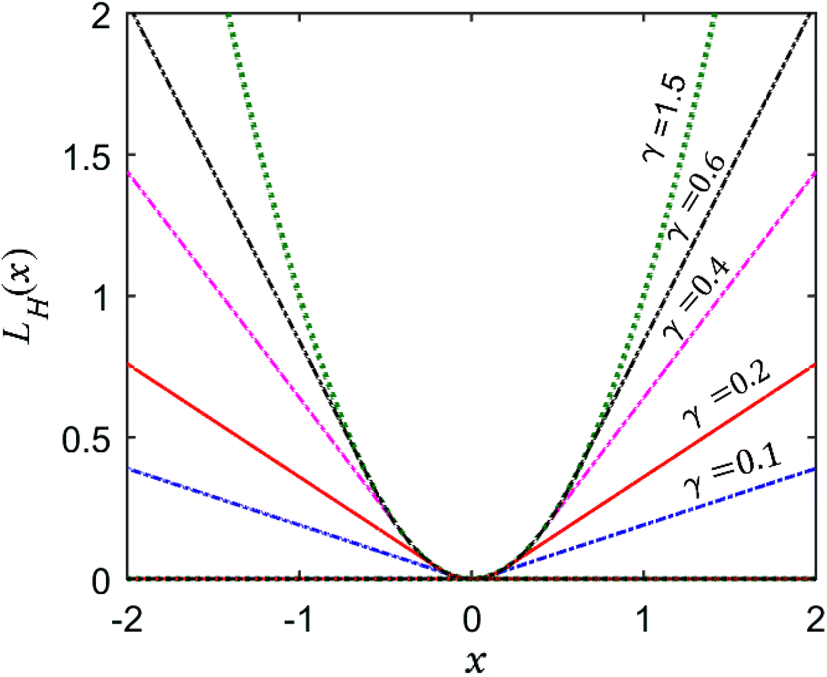
\includegraphics[width=0.8\linewidth]{HuberLoss}
			\end{figure}
		\end{column}
	\end{columns}
	
\end{frame}



\begin{frame}{Các bước huấn luyện với OHGesture}
%	\small
	\begin{enumerate}
		\item  Lấy nhãn $\bx_0$ từ phân bố của dữ liệu đã chuẩn hóa
		\item Tính sẵn các giá trị, và các siêu tham số: $\gamma$, $\sqrt{\alpha_t}$ $\sqrt{1 - \alpha_t}$, $\sqrt{\bar{\alpha}_t}$, Random nhiễu $\bepsilon_t$ ở mọi bước $t: 1 \rightarrow T$.
		$\{\alpha_t \in (0, 1)\}_{t=1}^T$
		\item Random Masks  $c_{1} = \big[ \mathbf{s} , \mathbf{e_1}, \mathbf{a}, \mathbf{v} \big]$, $c_{2} = \big[ \mathbf{s} , \mathbf{e_2}, \mathbf{a}, \mathbf{v}\big]$ hoặc $c_{2} = \big[ \varnothing , \varnothing, \mathbf{a},  \mathbf{v} \big]$
		\item Forward $\bx_0$ để có cử chỉ nhiễu $\mathbf{x}_t$ :  $\mathbf{x}_t = \sqrt{\bar{\alpha}_t}\mathbf{x}_0 + \sqrt{1 - \bar{\alpha}_t}\boldsymbol{\epsilon}_t$
		\item $\text{for all}$ $t$, lẫy $t$ \textbf{ngẫu nhiên} $t \sim [1, T]$
		\item Cho $\bx_t$ và $t$, $c$, $c_{\varnothing}$ để dự đoán chuỗi cử chỉ
		\begin{equation}
			\hat{\mathbf{x}}_{0 \gamma, c_{1}, c_{2}}=\gamma \cdot f_{\theta}  \left(\mathbf{x}_{t}, t, c_{1}\right)+(1-\gamma) \cdot f_{\theta} \left(\mathbf{x}_{t}, t, c_{2}\right)
		\end{equation}
%		 $\hat{\mathbf{x}}_0 =G_{\theta} (\mathbf{x}_t, t, c)$, $\hat{\mathbf{x}}_0^{\varnothing} =G_{\theta} (\mathbf{x}_t, t, c_{\varnothing})$

		\item Tính loss và đạo hàm để cập nhật trọng số $\theta$
		\begin{equation}
			\mathcal{L}_t = \mathbb{E}_{t \sim [1, T], \mathbf{x}_0, \boldsymbol{\epsilon}_t} \Big[ \operatorname{HuberLoss}(\mathbf{x}_0, \hat{\mathbf{x}}_0 ) \Big]
		\end{equation}
	
%	Trong đó $\mathbf{x}_t = \sqrt{\bar{\alpha}_t}\mathbf{x}_0 + \sqrt{1 - \bar{\alpha}_t}\boldsymbol{\epsilon}_t$
	
		\item Quay lại bước 6 cho đến khi hội tụ để thu được $\theta'$
	\end{enumerate}
\end{frame}


%\begin{frame}{}
%%	Mục tiêu: Áp dụng mô hình Diffusion cho vector tiềm ẩn:
%	1. Forward process:
%	$$
%	x_t = \sqrt{\alpha_t}x_0 + \sqrt{1-\alpha_t}\epsilon, \text{ where } \epsilon \sim \mathcal{N}(0,1)
%	$$
%	
%	2. Model prediction
%	- Input: $x_t$
%	- Output: $\hat{x}_0$ (predicted clean motion)
%	- Conversion between $\hat{x}_0$ and $\hat{\epsilon}$:
%	$$
%	\hat{\epsilon} = \frac{x_t - \sqrt{\alpha_t}\hat{x}_0}{\sqrt{1-\alpha_t}}
%	$$
%	
%	$$\hat{x}_0 = \frac{x_t - \sqrt{1-\alpha_t}\hat{\epsilon}}{\sqrt{\alpha_t}}$$
%	
%	3. Loss
%	$$\mathcal{L} = \| x_0 - \hat{x}_0\|^2 \text{ or } \|\epsilon - \hat{\epsilon}\|^2$$
%
%4. Sampling (Inference):
%	$$x_{t-1} = \sqrt{\alpha_{t-1}}\hat{x}_0 + \sqrt{1-\alpha_{t-1}-\sigma_t^2}\hat{\epsilon} + \sigma_t z$$
%%	\begin{figure}
%%		\centering
%%		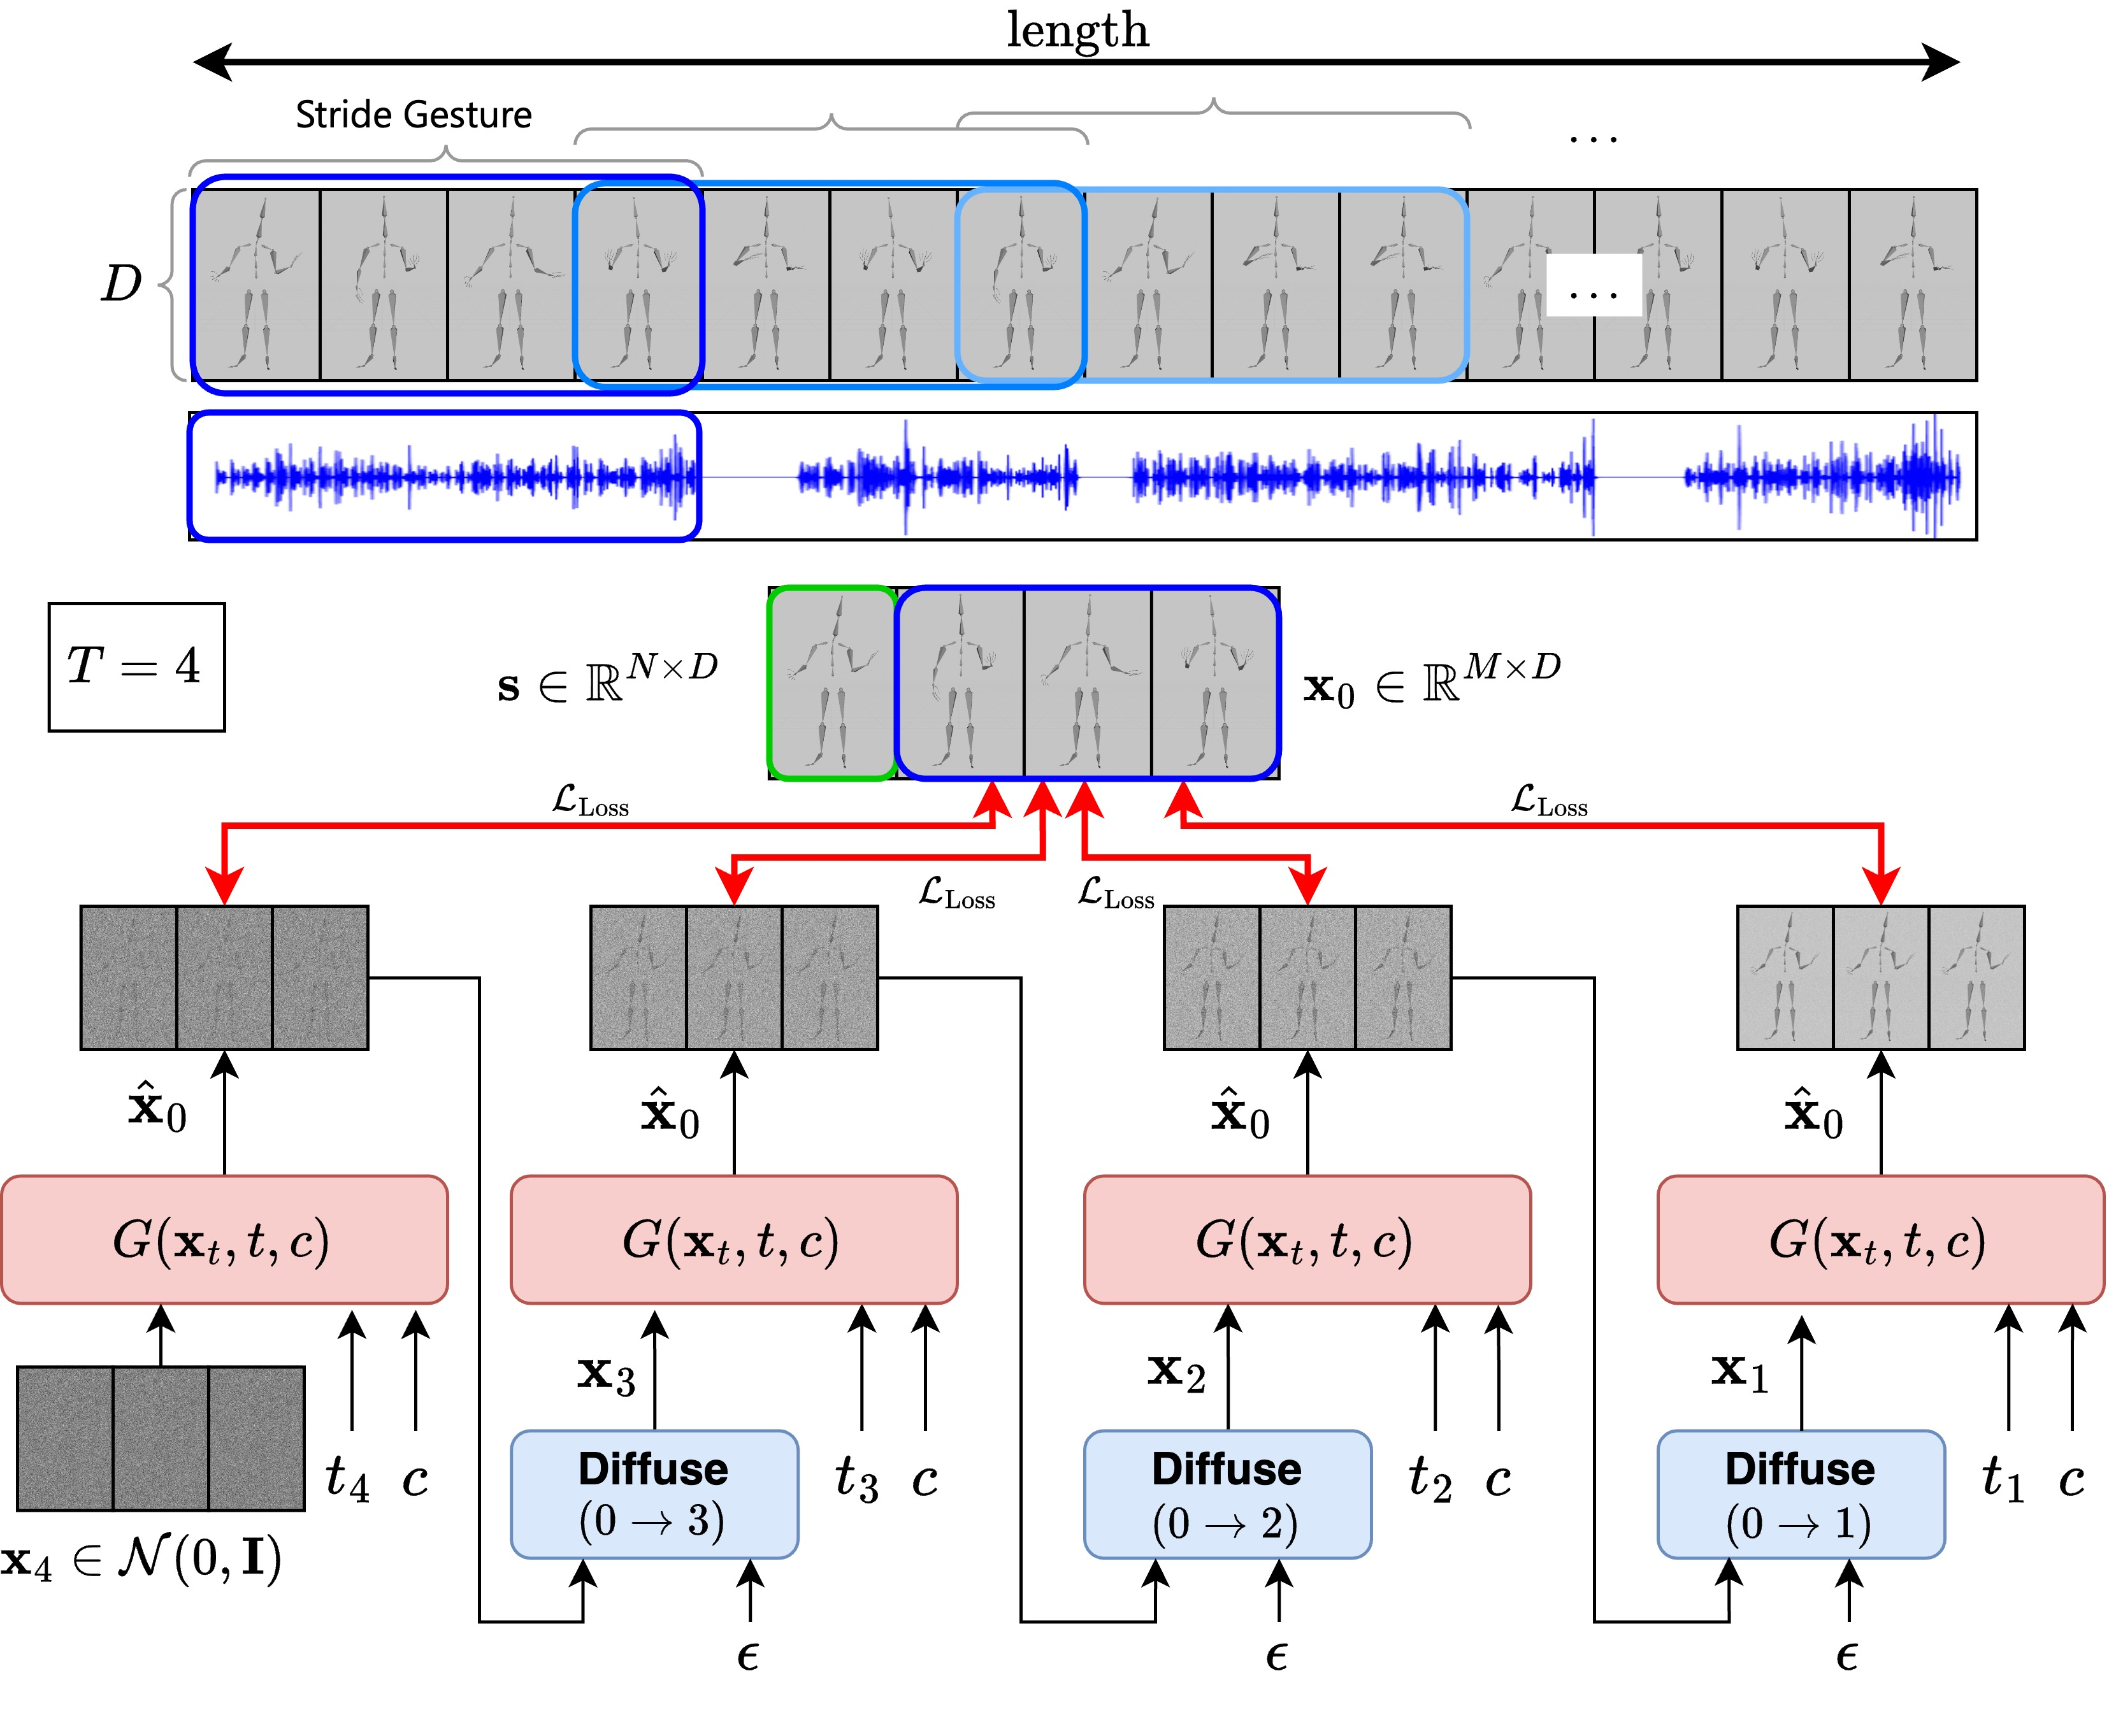
\includegraphics[width=\linewidth]{OverviewArchitecture}
%%	\end{figure}
%	
%\end{frame}
%OverviewConditionDiffusion



\begin{frame}{Các bước lấy mẫu (Sampling) với OHGesture}
	
	\begin{enumerate}
		\item Bắt đầu với nhiễu: $\bx_T \sim \mathcal{N}(0, \mathbf{I})$
		\item Các giá trị $\sqrt{\alpha_t}$ $\sqrt{1 - \alpha_t}$ và $\sqrt{\bar{\alpha}_t}$ có được từ bước huấn luyện, tính sẵn các giá trị  $\sigma_t$ từ $\alpha_t$ ở mọi bước $t: 1 \rightarrow T$
		\item Cử chỉ khởi tạo $\mathbf{s}$ ban đầu là trung bình dữ liệu, sau đó được lấy từ đoạn cử chỉ đã suy luận. Chọn cảm xúc mong muốn, văn bản được lấy từ transribe speech $\mathbf{a}$ và tạo cặp condition $c = [\mathbf{s}, \mathbf{e}, \mathbf{a},  \mathbf{v}]$
		\item $\text{for all}$ $t$, lấy $t$ \textbf{tuần tự} $t \sim [T, \dots 1]$
		\item Random nhiễu $\bz \sim \mathcal{N}(0, \mathbf{I})$
		\item Đưa $\bx_t$ vào để suy luận $\hat{\bx}_0^{(t)} = f_{\theta'}(\bx_t, t, c)$
		\item Forward $\hat{\bx}_0^{(t)}$ $0 \rightarrow t$ để được $\hat{\bx}_{t-1}^{(t)}$
		\item Cộng thêm một lượng nhiễu $\hat{\bx}_{t-1} = \hat{\bx}_{t-1}^{(t)} + \sigma_t \bz$
		\item Quay lại bước $4$, khi $t=1$ ta thu được $\hat{\bx}_0$ từ quá trình khử nhiễu
	\end{enumerate}
\end{frame}

\begin{frame}{Giai đoạn 7: Kết xuất (Render)}
\begin{figure}
		\centering
		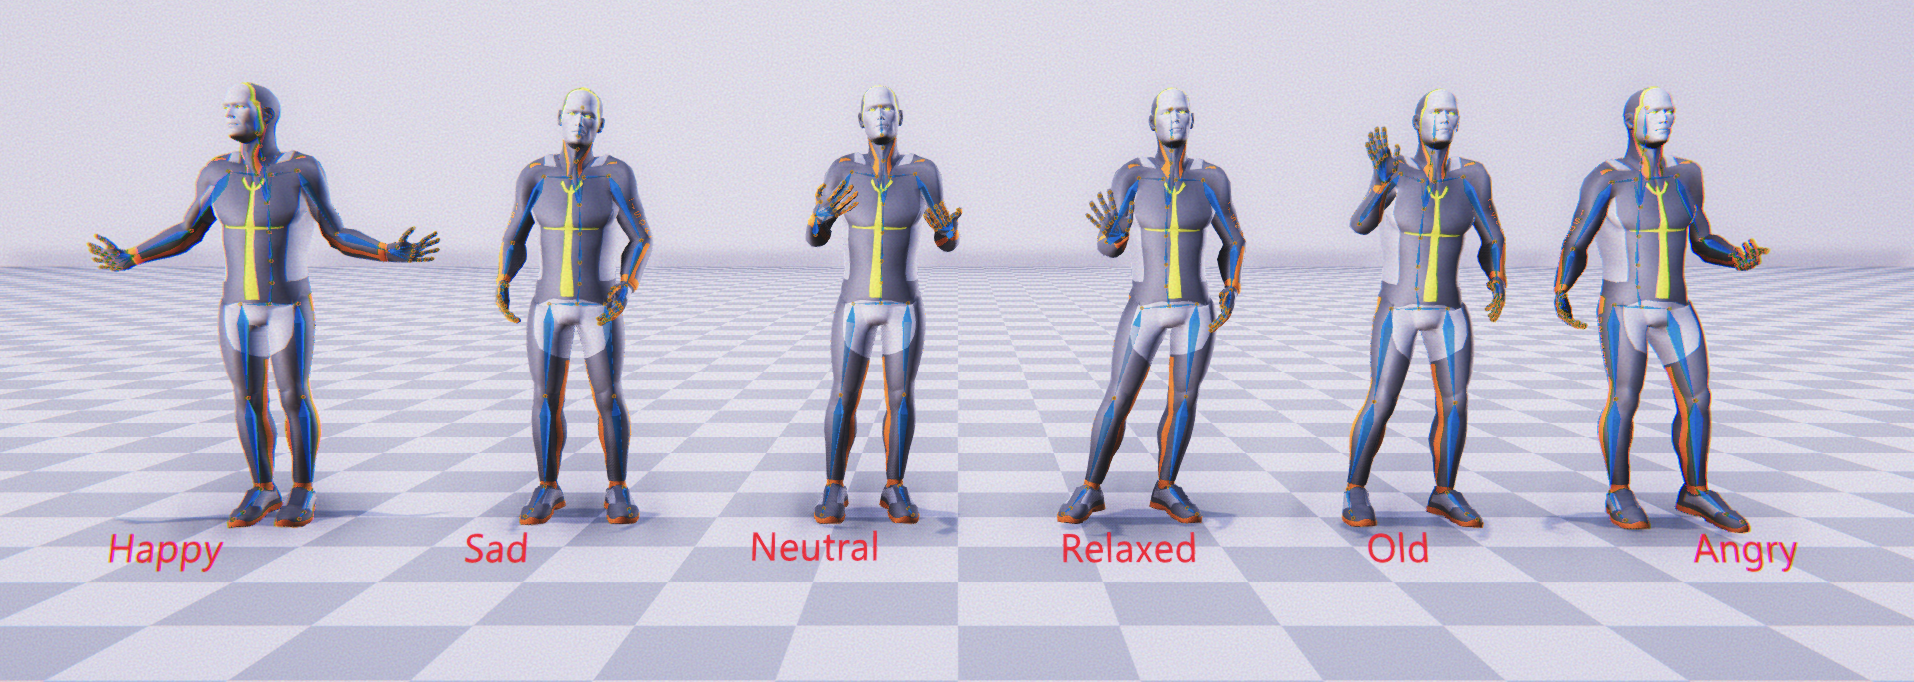
\includegraphics[width=\linewidth]{EmotionAnimation}
\end{figure}
\end{frame}
%\begin{frame}
%	\begin{figure}
%		\centering
%		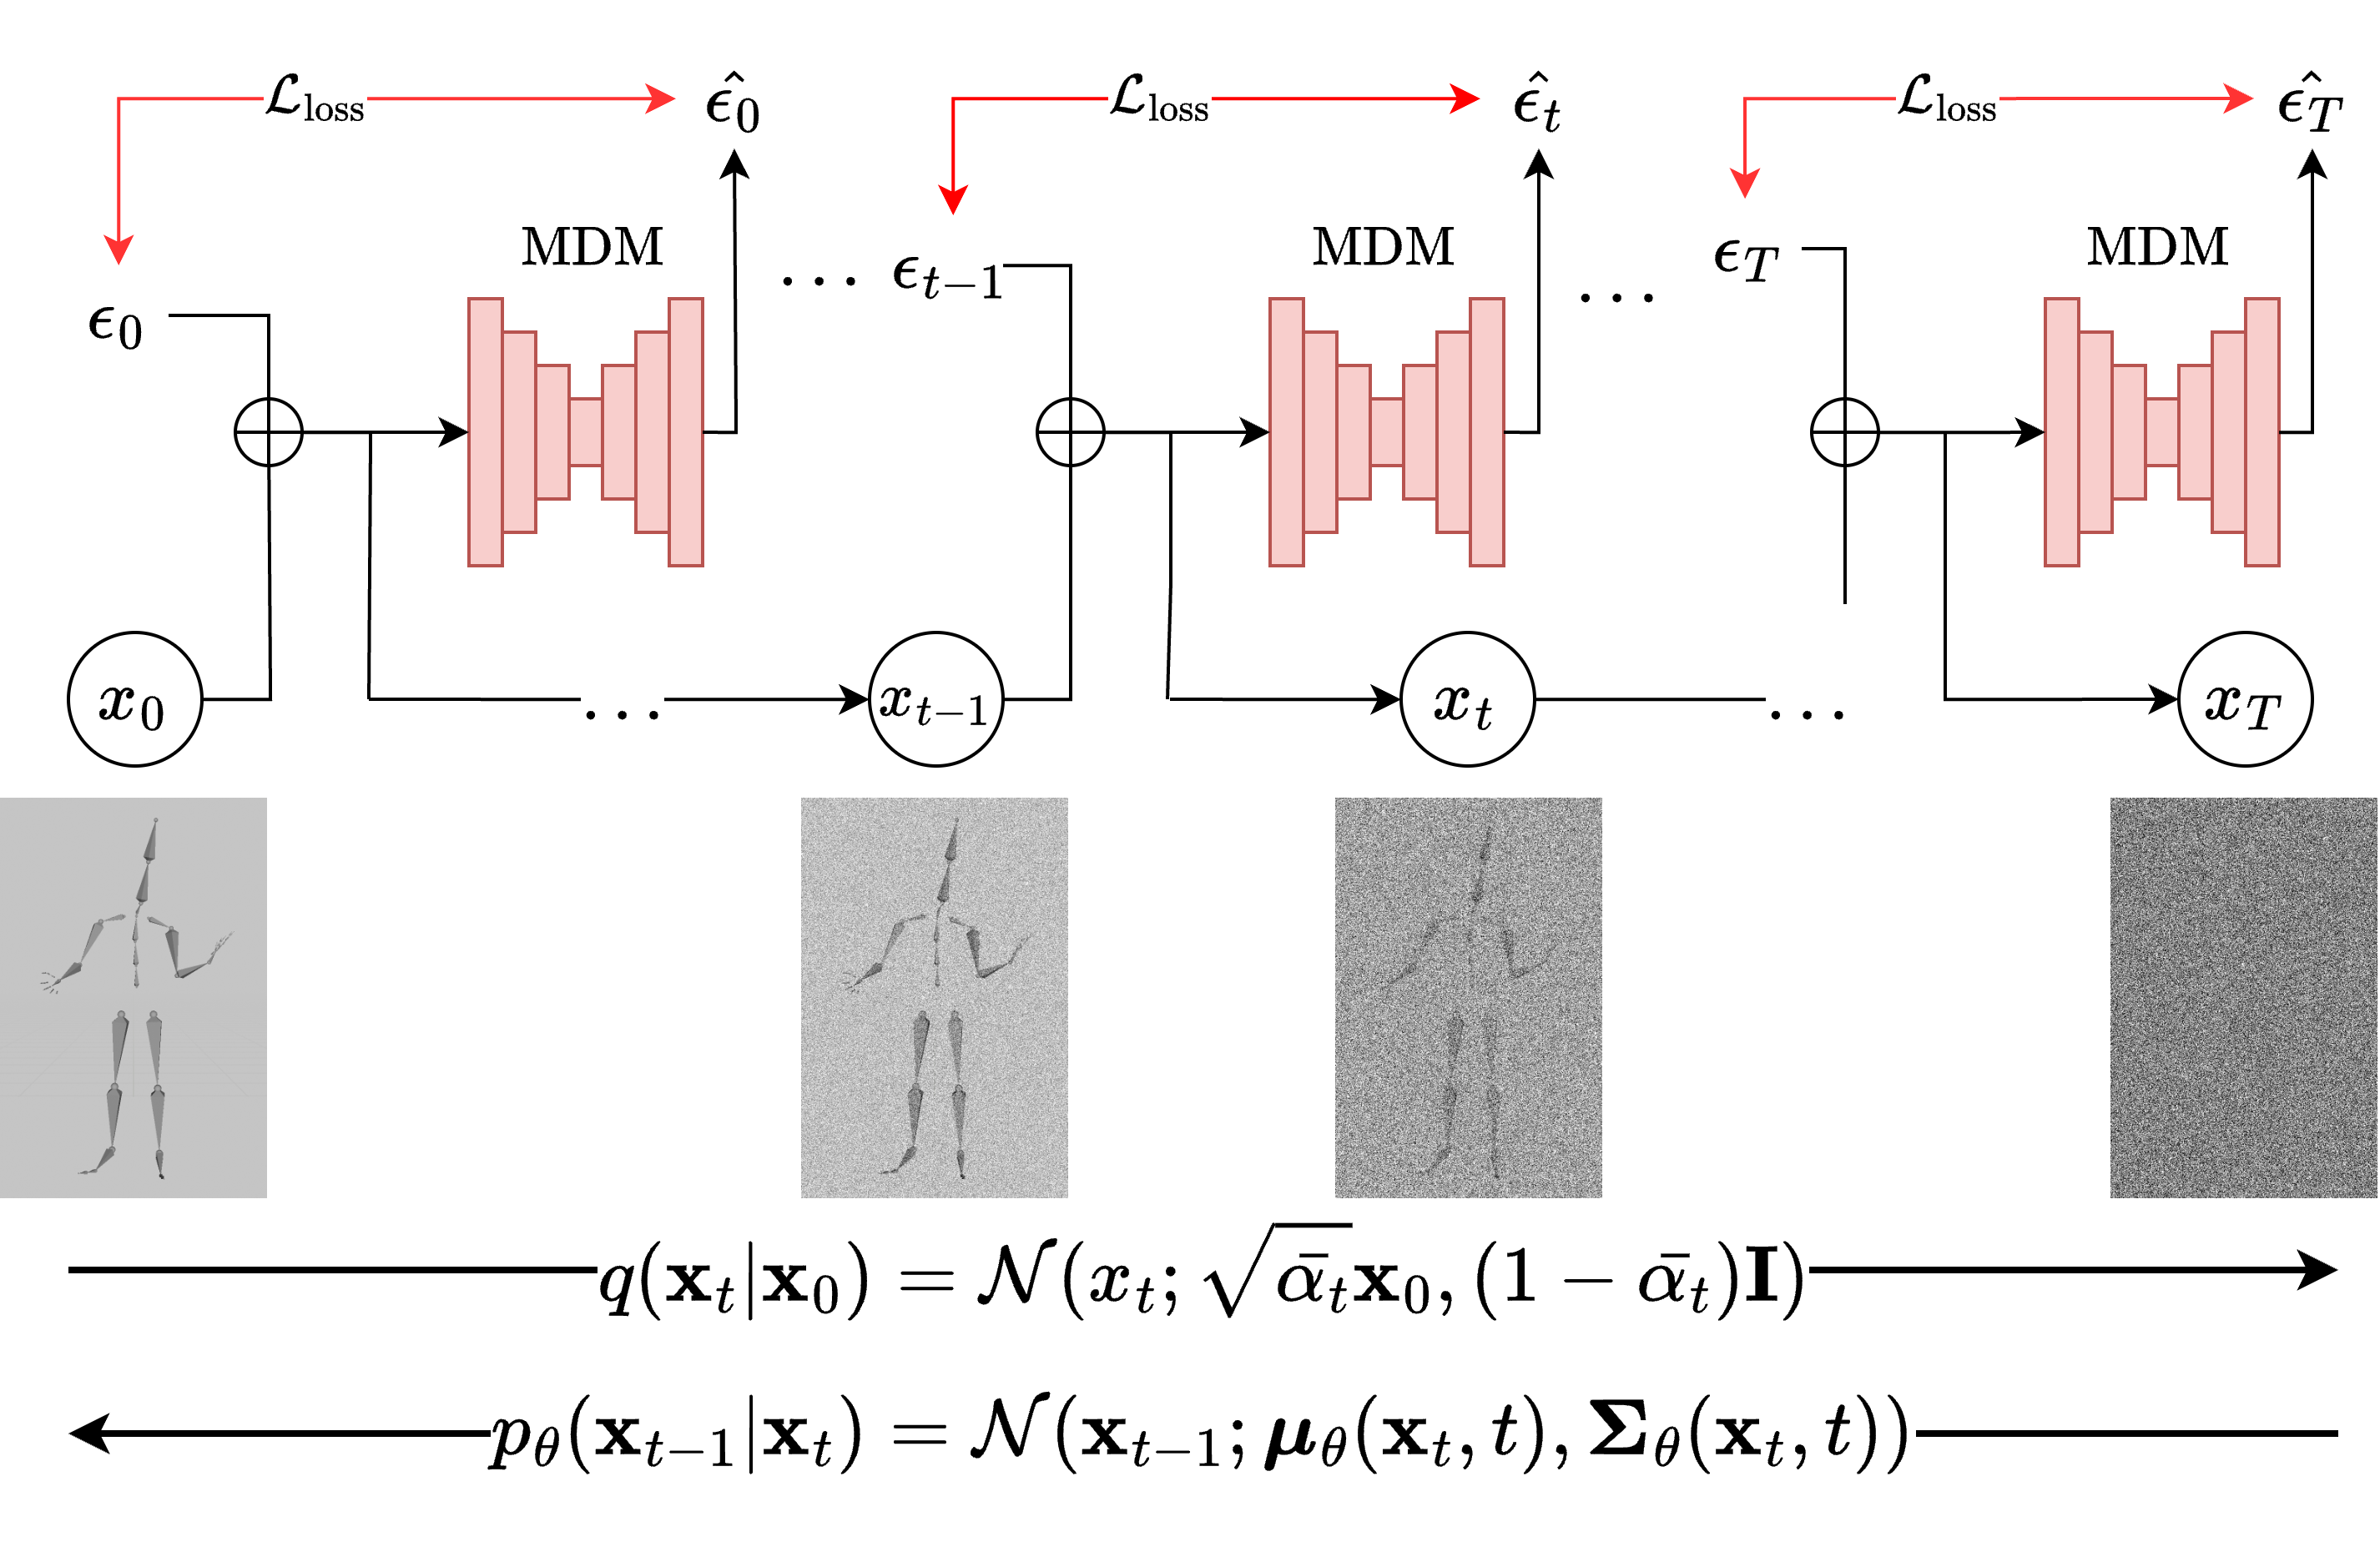
\includegraphics[width=0.8\linewidth]{DiffusionProcess}
%	\end{figure}
%\end{frame}


%\begin{figure} 
%	\centering
%	\includegraphics[width=0.8\linewidth]{DiffusionForward}
%\end{figure}


%\begin{frame}
%	
%	$
%	\label{Gaussian}
%	q\left(x_t \mid x_{t-1}\right)=\mathcal{N}\left(x_t ; \sqrt{1-\beta_t} x_{t-1}, \beta_t \mathbf{I}\right)
%	$
%	
%	$
%	\label{eq1}
%	q\left({x}_{1:T} \mid {x}_0\right)=\prod_{t=1}^T q\left({x}_t \mid {x}_{t-1}\right)
%	$
%	$
%	p_\theta\left({x}_{t-1} \mid {x}_t\right)=\mathcal{N}\left({x}_{t-1} ; {\mu}_\theta\left({x}_t, t\right), {\Sigma}_\theta\left({x}_t, t\right)\right)
%	$
%	
%	$
%	q\left({x}_t \mid {x}_0\right)=\mathcal{N}\left({x}_t ; \sqrt{\bar{\alpha}_t} {x}_0,\left(1-\bar{\alpha}_t\right) \mathbf{I}\right)
%	$
%	
%	$
%	\hat{x}_0=G\left(x_t, t, c\right)
%	$
%\end{frame}

	
%	\begin{columns}
	%		\begin{column}{0.5\textwidth}
		%			\textbf{DDPM (stochastic sampling):}
		%			\begin{itemize}
			%			\item Predict $x_0$ from $x_t$
			%			
			%			\item Convert to $\epsilon_{pred}$
			%			
			%			\item Use the formula:
			%			
			%			$$x_{t-1} = \frac{1}{\sqrt{\alpha_t}} x_t - \frac{1-\alpha_t}{\sqrt{1-\bar{\alpha}t}\sqrt{\alpha_t}} \epsilon_{\text{pred}} + \sigma_t z$$
			%			
			%			\item where $z \sim \mathcal{N}(0,I)$ is random noise
			%			\end{itemize}
		%			
		%		\end{column}
	%		
	%		\begin{column}{0.5\textwidth}
		%			\textbf{DDIM (deterministic sampling):}
		%			
		%			Predict $x_0$ from $x_t$
		%			
		%			NO additional noise term ($\sigma_t = 0$)
		%			
		%			Use the formula:
		%			
		%			$x_{t-1} = \sqrt{\bar{\alpha}{t-1}} x_0^{\text{pred}} + \sqrt{1-\bar{\alpha}_{t-1}} \epsilon_{\text{pred}}$
		%			
		%			Where:
		%			\begin{itemize}
			%			\item $\bar{\alpha}_t$ is the cumulative product of $\alpha$'s from 1 to t
			%			\item $\epsilon_{pred}$ is derived from $x_0$ prediction using:
			%			\item $\epsilon_{pred} = \frac{x_t - \sqrt{\alpha_t}x_{0_{pred}}}{\sqrt{1-\alpha_t}}$
			%			\end{itemize}
		%		\end{column}
	%	\end{columns}
	
